\section{RESULTS}
\label{sec:results}

\subsection{Investigation of off-diagonal elements}
\label{sec:off-diagonal-elements}

Before proceeding to the analysis of local chemical disorder effects on the magnetic damping, a natural question that arises -- linked to the tensorial character of $\alpha$ -- is about the practical contribution coming from the off-diagonal elements in a heterogeneus environment. In pure bcc or fcc $3d$ ferromagnets, when the spin quantization axis (SQA) aligns with a fourfold or threefold symmetry axis (e.g., in $\mathbf{z}$ direction), only diagonal elements are expected to be non-zero in the Gilbert damping tensor, as discussed in Refs. \cite{eriksson2017atomistic,PhysRevB.72.064450,PhysRevMaterials.2.013801} and corroborated by \cite{PhysRevB.108.014433}. This situation becomes ideal to extract a scalar $\alpha_{ij}$, which can be defined as $\alpha_{ij}=\frac{1}{2}\left(\alpha_{ij}^{xx}+\alpha_{ij}^{yy}\right)$, and to directly compare to what is typically measured in experiments \cite{PhysRevB.108.014433}. However, when considering an alloy with explicit chemical disorder, the intrinsic symmetry is broken, rendering non-zero off-diagonal elements plausible, even with SQA$\parallel\mathbf{z}$.

To address this problem, we considered the effective off-diagonal terms $\alpha^{\textnormal{eff}}_{xy}$ and $\alpha^{\textnormal{eff}}_{yx}$ (see Eq. \ref{eq:effective-tensor-elements}) from a bcc special quasirandom structure containing 16 atoms (SQS-16) \cite{Zunger1990}, obtained for a particularly simple FeCo concentration (Fe$_{50}$Co$_{50}$). The SQS-16 cell was created using the MCSQS algorithm within the framework of the Alloy Theoretic Automated Toolkit (ATAT) \cite{vandeWalle2013}; more details on the method inputs to create the cell can be found in Ref. \cite{PhysRevB.108.014433}.

Clearly, the off-diagonal terms do not vanish (see Fig. \ref{fig:off-diag-sqs} in the Appendix \ref{sec:off-diagonal-convergence}), but they represent a very small fraction of the diagonal terms ($\sim4-5\%$). Also, the asymmetry is reduced between the diagonal terms ($\sim2\%$), which indicates that at large scales the chemical disorder plays a smaller role on the format of the $\hat{\alpha}^{\textnormal{eff}}$ tensor than the symmetry of the bcc structure in connection with the SQA itself. In other words, it is a decent approximation to consider $\alpha^{\textnormal{eff}}\rightarrow\frac{1}{2}(\alpha_{xx}^{\textnormal{eff}}+\alpha_{yy}^{\textnormal{eff}})\sim\alpha_{xx}^{\textnormal{eff}}$. Therefore, although locally off-diagonal elements maybe not negligible, we can consider in our investigation only the average $\alpha_{ij}=\frac{1}{2}\left(\alpha_{ij}^{xx}+\alpha_{ij}^{yy}\right)$, that will effectively contribute to $\alpha^{\textnormal{eff}}$ in the bulk scale.


\subsection{Local effects: the Fe$_{87}$Co$_{13}$ case}
\label{subsec:local-effects-detailed}

Contrary to the Heisenberg exchange, which shows an isotropic nature in the collinear state (i.e., dependent on the atomic pair distance, and without the SQA as a symmetry reducer), the Gilbert damping is anisotropic with respect to the SQA -- even within the same neighboring shell. Formally, while the former is explained by a simultaneous conservation of the trace of the block Green's functions $\hat{G}_{ij}$ (and, consequently, also $\hat{A}_{ij}$) and $\ell$-dependent diagonal exchange-splitting matrices (see, e.g., \cite{PhysRevB.62.5293,PhysRevB.91.125133}), the later is explained by the non-diagonal character of the torque operators $\hat{T}_i^{\mu}$ (Eq. \ref{eq:damping-dft}). In other words, not only the distance and chemical classification of the $ij$-pair is important for the composition of $\alpha_{ij}$ values, but also their position with respect to the SQA (throughout the text we consider $\textnormal{SQA}\parallel\mathbf{z}$ -- unless otherwise noted). Physically, this can be understood by two connected facts: (\textit{i}) for small rotations of the spin about the SQA ($\mathbf{z}$), if it is a high symmetry axis,  the change in the magnetization will stay confined in the other two independent reference orientations ($\mathbf{x}$-$\mathbf{y}$ plane in this case, so $\mu\in\{x,y\}$), and (\textit{ii})  the spin-orbit torques will recruit different contributions from the orbitals in the inter-site electronic spectral functions (i.e., through $\hat{A}_{ij}$) to participate in the dissipation process, obeying their symmetries in real-space. This anisotropic behavior of $\alpha_{ij}$ has been observed and reported in Refs. \cite{PhysRevB.103.L220405,PhysRevB.108.014433,PhysRevMaterials.2.013801}, where sometimes more than a single value of non-local damping is found for the same inter-site distance $r_{ij}$, even for single-element materials. As an example, we can analyze the second neighboring shell of (pure) bcc Fe, which presents two distinct $\alpha_{ij}$ values \cite{PhysRevB.108.014433}. In this case, the orbital symmetry of the sites localized at positions $(\pm a_0,0,0)$ and $(0,\pm a_0,0)$ ensure a swap between $\alpha_{ij}^{xx}$ and $\alpha_{ij}^{yy}$ in the respective $\hat{\alpha}_{ij}$ tensors, resulting in the same $\alpha_{ij}$ parameters according to the definition in Section \ref{sec:methods}. However, the sites localized at positions $(0,0,\pm a_0)$ are characterized by inter-site propagators $\hat{G}_{ij}$ with completely different (diagonal and non-diagonal) orbital contributions, resulting also in distinct $\hat{\alpha}_{ij}$ tensors when compared to the previous 4 sites. Unfortunately, the non-diagonal character of the $\hat{T}_i^{\mu}$ operators prevents us from discretizing the diagonal $\alpha_{ij}^{\mu\nu=\mu}$ elements in orbital contributions in a simple and analogous way as for the Heisenberg exchange interactions ($J_{ij}$'s, see Refs. \cite{PhysRevB.91.224405,PhysRevLett.116.217202}).

Given the complexity associated with the set of degrees of freedom that potentially influence the real-space $\alpha_{ij}$'s (chemical classification, distance, and position around a SQA), the best possible scenario to investigate local effects is to consider all configurations for the particular alloy concentration of interest. In this context, as a bonus, not only local effects can be studied, but also explicit alloying disorder (short-range disorder) can be indirectly considered as one source of electronic finite lifetime in these materials \cite{PhysRevB.87.014430} -- generally treated by effective medium approaches, such as the simple VCA \cite{PhysRevB.108.014433} or the more accurate CPA \cite{PhysRevB.87.014430,PhysRevB.98.174412,PhysRevLett.105.236601,PhysRevB.92.214407}.  In a 15-atom cluster, with $p$ number of Co atoms inside the cluster, this means a total number of configurations equal to $C^{15}_{p}=\binom{15}{p}=\frac{15!}{p!(15-p)!}$ for a given concentration Fe$_{{100-\frac{20p}{3}}}$Co$_{\frac{20p}{3}}$.

As this result scales quickly to thousands of possible configurations, we can choose an Fe-rich alloy to be our proof-of-concept, i.e., we choose $p=2$ (or Fe$_{87}$Co$_{13}$). In this case, the 105 total configurations can be reduced to 16 nonequivalent situations, following the symmetry of the Gilbert damping parameters in the bcc structure. However, before we analyze the average on this alloy, we discuss in detail a single case among the 16 nonequivalent situations.

\begin{figure}[!ht] 
\centering
        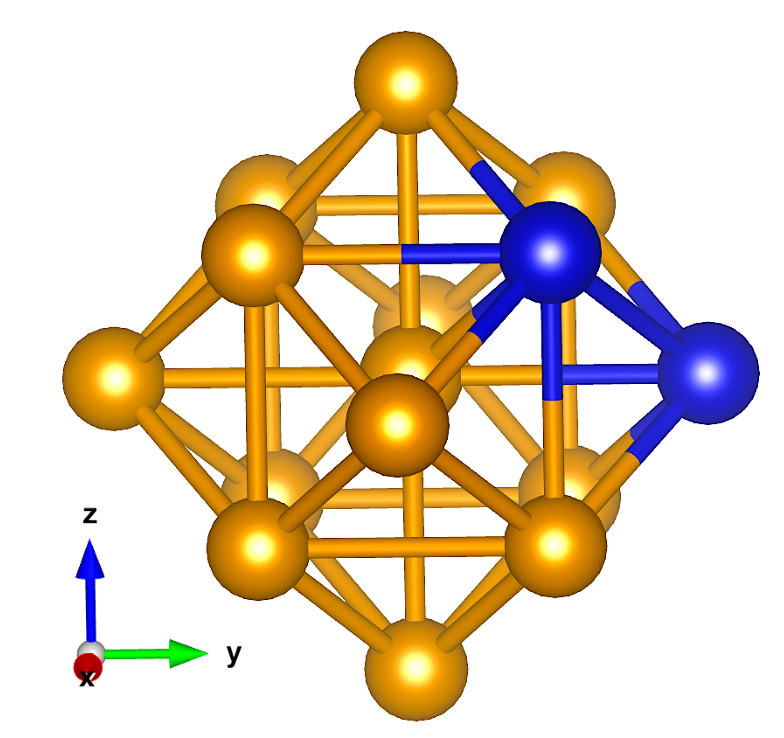
\includegraphics[width=0.6\columnwidth]{Fig3.png}
        \caption{(Color online) Schematic representation of a 15-atom embeddedcluster with alloy concentration Fe$_{87}$Co$_{13}$. Within the EC-VCA model, this figure depicts only the explicit part, which in the calculations is surrounded by the corresponding VCA medium. The color scheme of the spheres is consistent with Fig. \ref{fig:ec-vca-representation}. Bonds are drawn to guide the eye. Image produced with the VESTA software \cite{Momma2011}.}
        \label{fig:cluster-example} 
\end{figure}

As an example, consider the cluster displayed in Figure \ref{fig:cluster-example}. In principle, due to the cubic environment, each of the $\{\mathbf{x},\mathbf{y},\mathbf{z}\}$ axes present a 4-fold ($C_4$) symmetry with respect to the $\alpha_{ij}$ values, representing a total of 24 non-equivalent configurations (from the initial 105). However, in view of the reasons discussed above, when a Co atom occupies any site within the SQA ($\mathbf{z}$-axis), the $\alpha_{\textnormal{Fe-Co}}$ value is distinct, reducing the multiplicity of this example to 16. In that case, the variation of the nearest-neighbor Co position w.r.t. the central Fe atom do not change the $\alpha_{ij}^{\mu\nu}$ components, but the second nearest-neighbors (NNN), even when occupied by Co atoms, follow the same symmetry rules as the pure bcc Fe (swap $\alpha_{ij}^{xx}\leftrightarrow\alpha_{ij}^{yy}$ for NNN in the $xy$-plane, different components for NNN in $\mathbf{z}$). 

We can quantify the difference for this example.  Taking into account the multiplicity, the variation in $\alpha_{i}$  (Eq. \ref{eq:damping_sum}, $r_c=6a_0$) of having Co in the $\mathbf{z}$-axis or in the $xy$-plane amounts to $\sim1\%$ -- similarly to other quasi-equivalent cases among the 16 configurations. That is not a purely non-local effect, as the onsite contribution also varies with about the same intensity. Although small for Fe-Co alloys, given their relatively weak spin-orbit strength, we anticipate that the variation in $\alpha_{i}$ is larger for environments with higher spin-orbit coupling, $\xi$, in the limit where the adiabatic and mean-field approximations (assumed for torque-correlation formalism used here) are still reasonable \cite{PhysRevB.92.014419}.

\begin{figure*}[!ht] 
\centering
        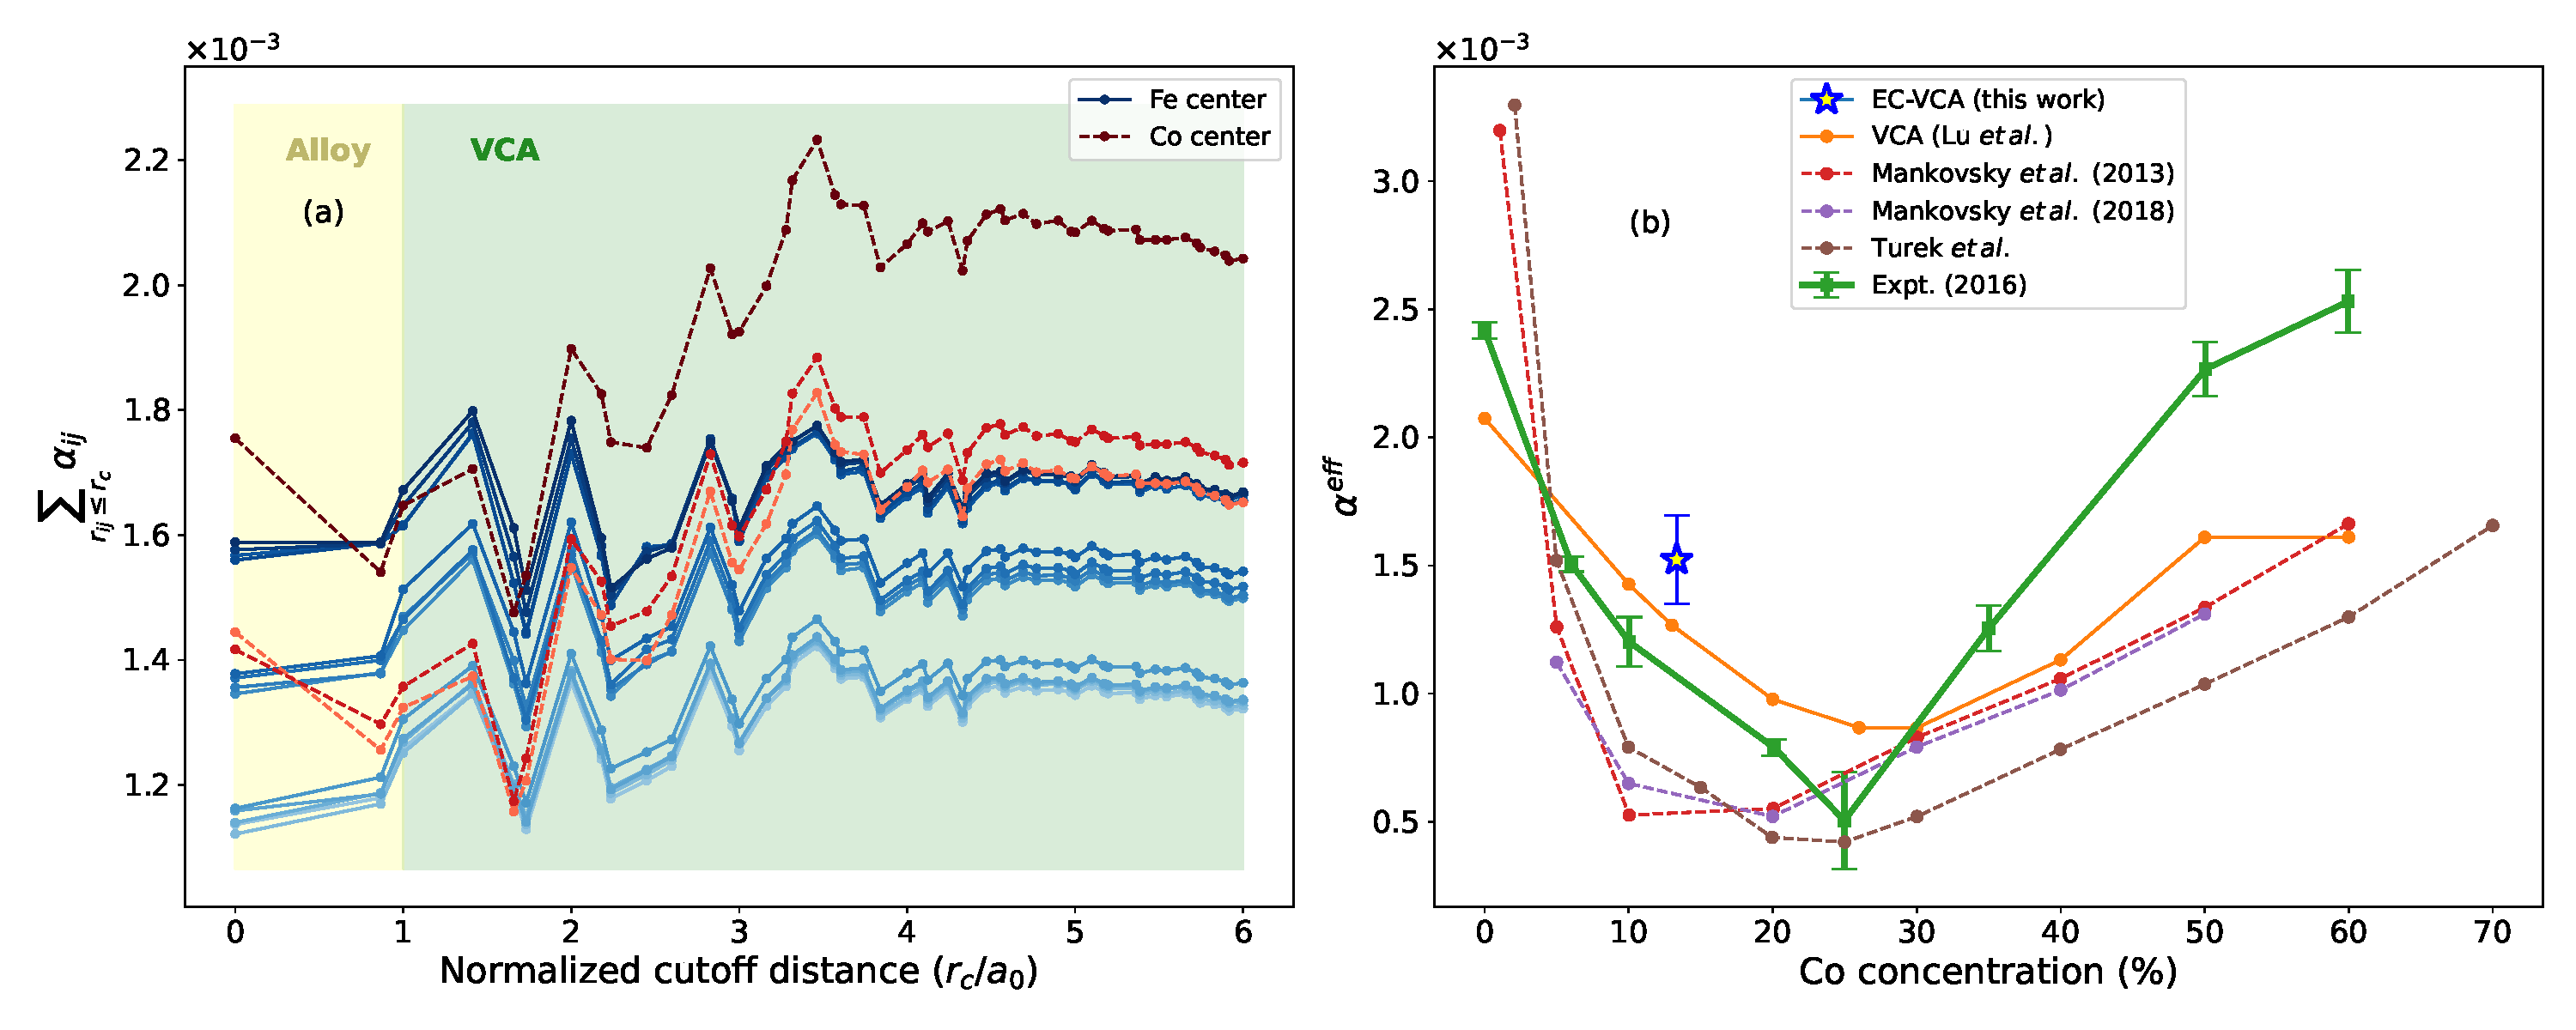
\includegraphics[width=\textwidth]{Fig4.pdf}
        \caption{(a)  $\sum_{r_{ij}\leq r_c}\alpha_{ij}$ up to a given cutoff radius ($r_c$) of all nonequivalent configurations of Fe$_{87}$Co$_{13}$ in the EC-VCA model. The different curves shown in colors with different shades of blue represent different Fe-centered clusters, while the curves shown with different shades of red show different Co-centered ones. (b) Comparison of the effective damping obtained from all Fe$_{87}$Co$_{13}$ configurations in the EC-VCA model (blue point) with theoretical values obtained by the use of effective medium approaches (VCA \cite{PhysRevB.108.014433}, and CPA \cite{PhysRevB.92.214407,PhysRevB.87.014430,PhysRevB.98.104406}) and with the experimental values of intrinsic damping \cite{Schoen2016}. In (a), the yellow and green areas represent the explicit alloy and VCA medium regions of the EC-VCA model, respectively.
        } 
        \label{fig:damping-fe87co13} 
\end{figure*}

It is instructive to analyze the damping that can be calculated from all possible nonequivalent configurations of Fe$_{87}$Co$_{13}$. The results of both individual cumulative damping summations (Eq. \ref{eq:damping_sum}), and comparison between the effective damping of Fe$_{87}$Co$_{13}$ and previous literature results are shown in Figure \ref{fig:damping-fe87co13}. We first notice from Fig. \ref{fig:damping-fe87co13}(a) that generally, the values of $\alpha_i$ for Co-centered clusters in the explicit alloy region are higher (scaling with $\frac{1}{m_i}$) than the Fe-centered ones, and also subject to more oscillations, especially throughout the VCA medium. More importantly, even within each set of Fe- or Co-centered configurations, we note the presence of distinct curves, which is a direct consequence of the different spatial distributions of Fe/Co inside the embedded cluster region -- or, in other words, a direct influence of the local environment. Although the onsite contribution ($\alpha_{ii}$) drives the majority of the effect, essentially due to changes in the local density of states around $E_F$ because of the charge transfer between species, the non-local contribution cannot be disregarded. This is partially in line with the importance of site-resolved non-local damping suggested in Ref. \cite{PhysRevB.109.094417}, although the authors indicate it in the context of reduced dimensionality -- and here we argue its relevance in the presence of short-range chemical disorder. Explicitly, the largest variation of the $\alpha_{ii}$ values among the Fe- and Co-centered clusters are $\sim4.7\times10^{-4}$ and $\sim3.4\times10^{-4}$, respectively, while the (pure) nonlocal contributions vary $\sim0.9\times10^{-4}$ ($\sim1.3\times10^{-4}$) and $\sim0.6\times10^{-4}$ ($\sim0.9\times10^{-4}$) for $r_c=a_0$ ($r_c=6a_0$), where $r_c=a_0$ represents the limit of the embedded cluster region.


With the definition given by Eq. \ref{eq:total-damping}, the effective Gilbert damping can be obtained. The comparison of $\alpha^{\textnormal{eff}}$ for Fe$_{87}$Co$_{13}$ with other literature results is shown in Fig. \ref{fig:damping-fe87co13}(b). The error bar, here identified as the precision of $\alpha^{\textnormal{eff}}$, is calculated by the standard deviation and evaluated as $\sim11\%$. This percentage will be used in a later stage as the approximate error of other Co concentrations averages. The final result of the EC-VCA model, $\alpha^{\textnormal{eff}}=(1.52\pm0.17)\times10^{-3}$, can then be compared to the pure VCA calculation, $\alpha^{\textnormal{eff}}=1.27\times10^{-3}$. Despite the consideration of almost the same chosen broadening parameter, $\delta$, the effective damping for the EC-VCA model is enhanced in comparison with the pure VCA value. This is partially related to the fact that the configuration average indirectly introduces the chemical disorder as a cause for change in $\delta$ (electronic lifetime), and the randomly arranged atoms as centers for electronic scattering. Another obvious reason associated with this difference, that cannot be neglected, is the relative small size of the embedded cluster. However, as Fig. \ref{fig:damping-fe87co13}(b) shows, both the VCA and EC-VCA calculatons capture most experimental results fairly well. 


\subsubsection{Spin dynamics: remagnetization}
\label{sec:explicit-asd}

The calculation of explicit $\alpha_{ij}$ parameters in the EC-VCA model allows for the inspection of the local environment effects on dynamical processes, in a fully atomistic picture. %This is particularly interesting for this problem. 
Although the impact of a 15-atom explicit region on the overall energy dissipation rate is expected to be small, the spin dynamics within this region can significantly differ from that obtained considering an array consisting solely of VCA sites. In this sense, the remagnetization stands as a suitable process to investigate; its relevance becomes evident in the context of, e.g., ultrafast pump-probe experiments and magnetization switching \cite{Radu2011,PhysRevLett.121.077204,Pankratova2024}, even though care should be taken in the direct comparison to those experimental results as variations in the spin moment length are not accounted for in the generalized LLG equation \cite{PhysRevB.109.094417,PhysRevMaterials.2.013801,PhysRevB.108.014433,PhysRevB.73.184427}.

With this aim, we assume minimal influence from off-diagonal elements (see Section \ref{sec:off-diagonal-elements}) and employ the method outlined in Ref. \cite{PhysRevB.108.014433}. As a test case, we examine the remagnetization dynamics with an embedded cluster as shown in Fig. \ref{fig:cluster-example}, starting from a random noncollinear state (same for all simulations). This dynamics with an explicit cluster can then be compared to the Fe$_{87}$Co$_{13}$ fully VCA model to account for the impact of the locally distinct nonlocal Gilbert dampings. In this context, the $J_{ij}$ set also differs. Thus, a third model in which all exchange interactions are artificially replaced by the corresponding VCA values is considered, to isolate the effect of $\alpha_{ij}$'s. All sets of computed $J_{ij}$ parameters, correspondent to both the pure VCA calculation and the EC-VCA model, are depicted in Appendix \ref{sec:jijs-sets-asd}.

Figure \ref{fig:explicit-asd}(a) shows the obtained average magnetic moments, considering both nonlocal and site-resolved effective damping descriptions, for all three models (pure VCA, EC-VCA, and EC-VCA with the VCA $J_{ij}$ set). The first point to be noted is the global decrease of the energy dissipation rate by the nonlocal damping formulation of the equation of motion ($\alpha_{ij}$, full lines) compared to the effective damping ($\alpha_i$, dashed lines). Moreover, all three models show distinct remagnetization times, as highlighted by the \textit{Insets}. For example, among the three models, we obtain maximum differences  of $\sim600$ fs and $\sim200$ fs to reach $\sim77\%$ of the fully saturated magnetization in the $\alpha_i$ and $\alpha_{ij}$ simulations, respectively; as these differences occur between the pure VCA and the EC-VCA with the same exchanged $J_{ij}$ set, they can be ascribed solely to the $\alpha_{ij}$'s. Interestingly, here the contrast between the nonlocal and effective descriptions is also evident: the dissipation rate of the pure VCA model is the highest in the former and the lowest in the latter.

Altogether, those results clearly demonstrate how the short-range disorder influence on the local dynamics can modify the overall relaxation rate. However, here the impact is reduced due to two main factors: (\textit{i}) the previously mentioned small replaced region in the VCA matrix (15-atom cluster in a $40\times40\times40$  lattice); and (\textit{ii}) the choice of a cluster whose effective damping (central atom $\alpha_i=1.32\times10^{-3}$) does not considerably deviate from the VCA value ($\alpha_i=1.27\times10^{-3}$). This suggests promising prospects for enhanced effects in larger embedded regions or in scenarios where damping varies significantly (up to an order of magnitude), as explored in the next section. It also corroborates with the assertion from Ref. \cite{PhysRevB.109.094417} that considering inhomogeneous damping can improve the accuracy of spin dynamics simulations.

To better illustrate the influence of chemical disorder on the local dynamics, in Fig. \ref{fig:explicit-asd}(b) we show the trajectories of both the central spin, which coincides with the center of the embedded cluster, and a peripheral spin located more than $6a_0$ from the center, encompassing only VCA-type interactions. Concerning the former, it is possible to see that the trajectories largely deviate in all three models from the beginning. In turn, for the latter, the dynamics only start to differ after a time interval of $\Delta t\sim 0.13$ ps, by the perturbation of spin waves coming from the cluster region.


\begin{figure*}[!ht] 
\centering
        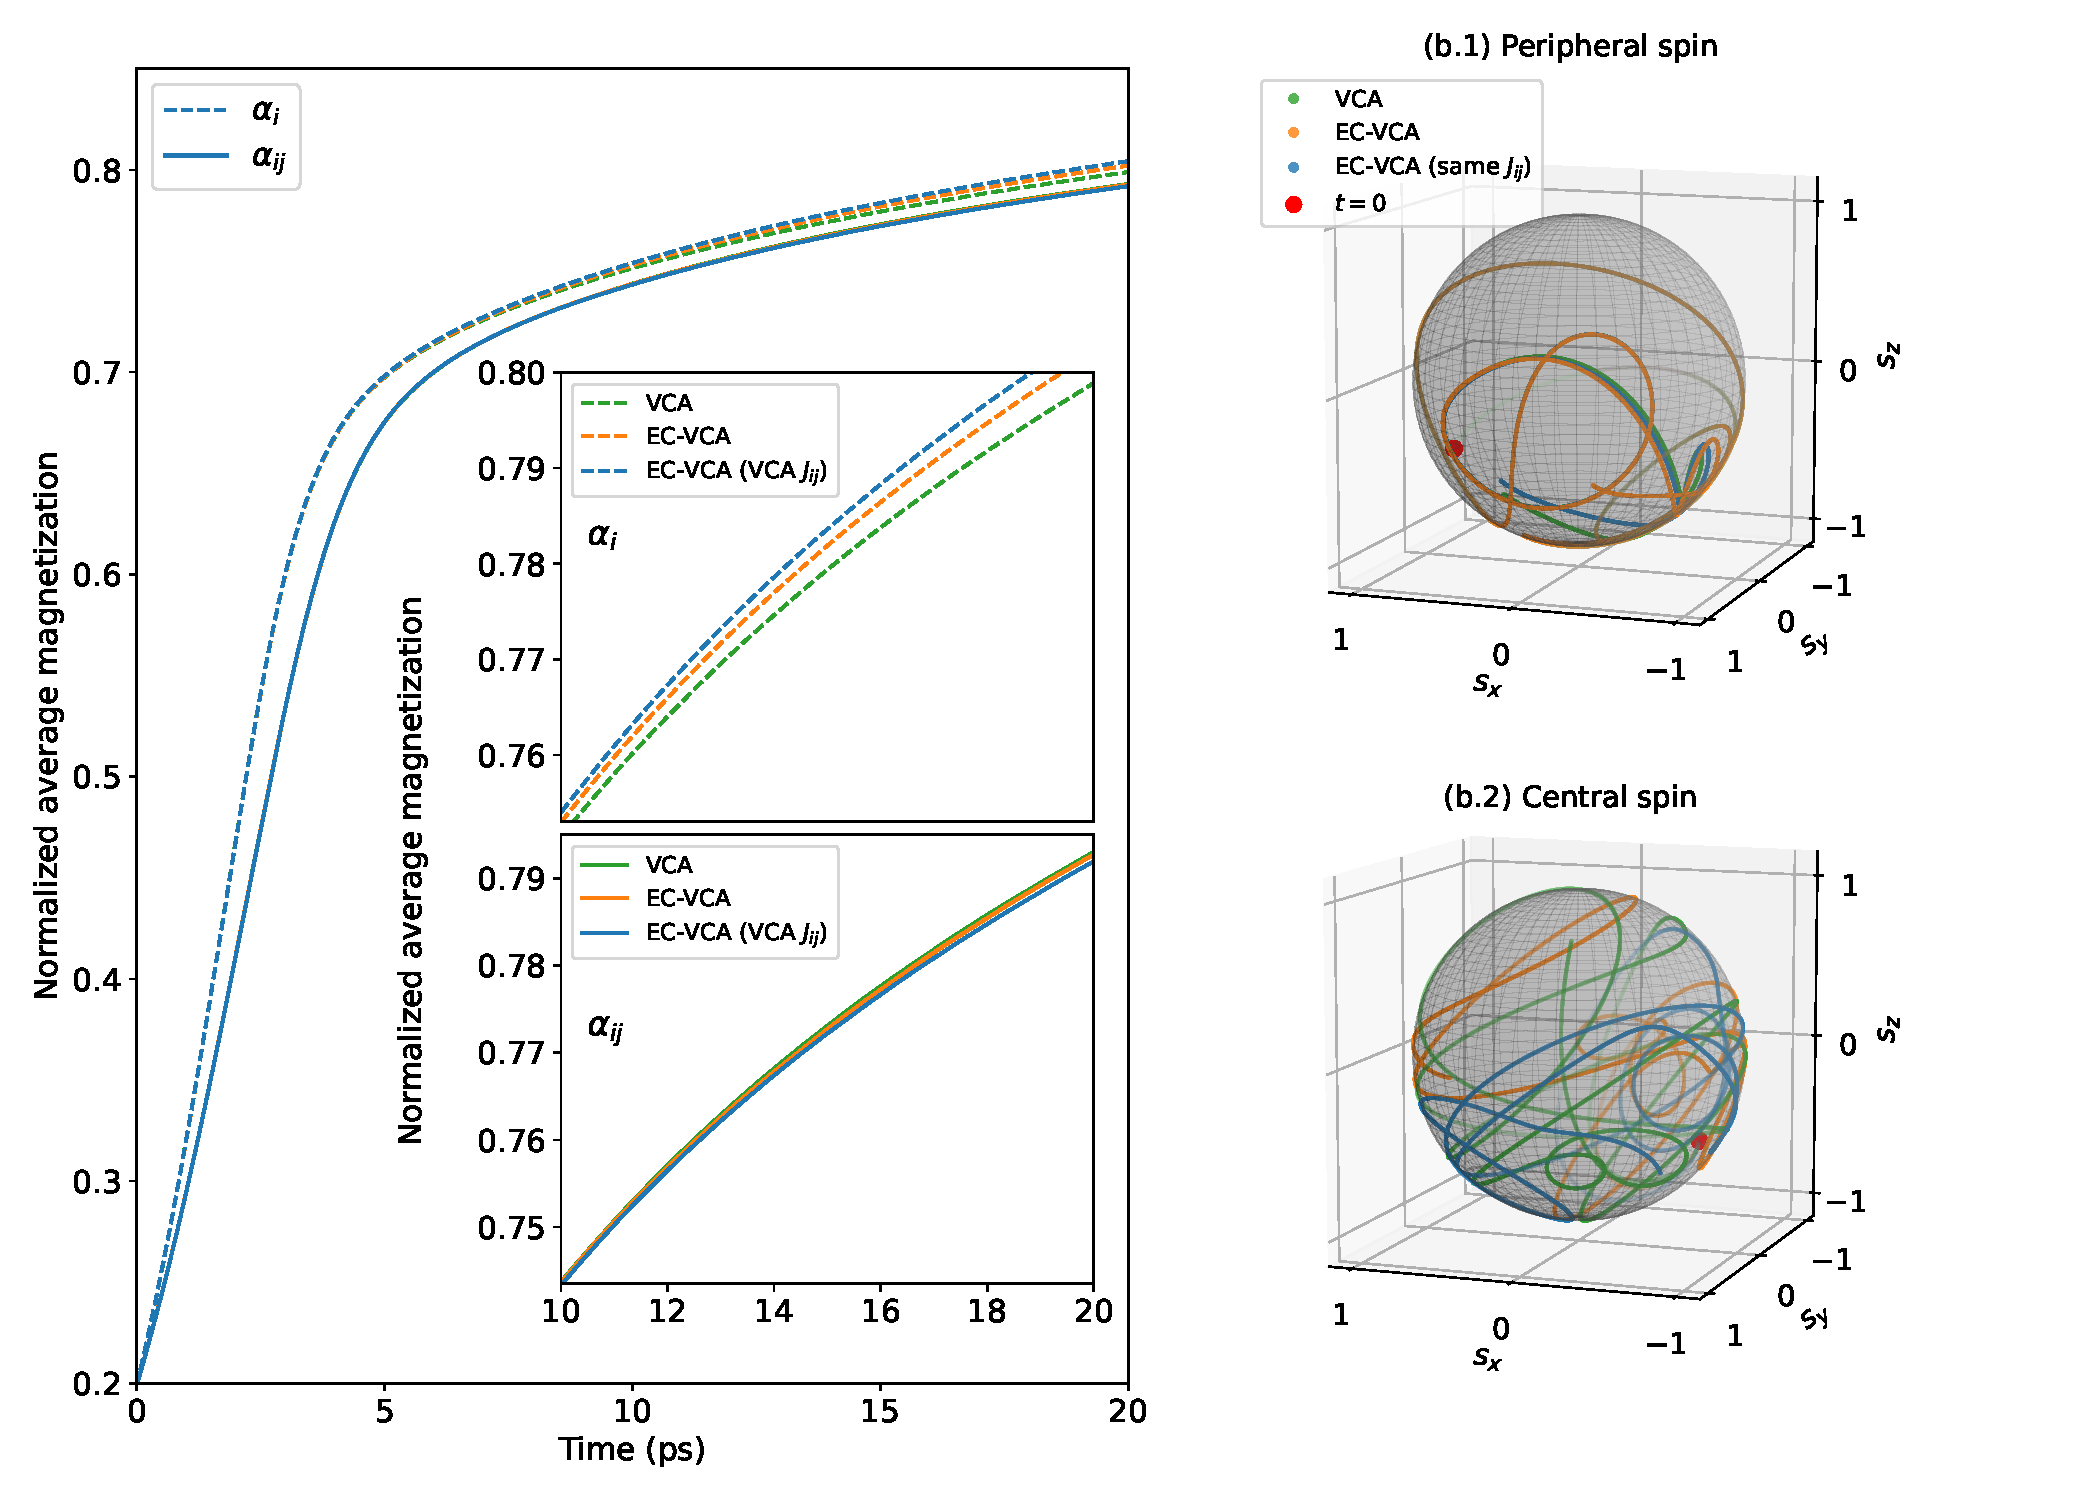
\includegraphics[width=0.9\textwidth]{Fig5.pdf}
        \caption{(a) Remagnetization process for Fe$_{87}$Co$_{13}$ simulated with atomistic spin dynamics, considering both the fully nonlocal Gilbert damping ($\alpha_{ij}$, solid lines) and the site-resolved effective damping ($\alpha_i$, Eq. \ref{eq:damping_sum}, dashed lines). Green, orange and blue lines symbolize the simulations performed with purely VCA, EC-VCA, and EC-VCA parameters considering the VCA $J_{ij}$ set, respectively. \textit{Insets:} a zoom-in of the normalized magnetization curves. (b) Spin trajectories lying on the unit sphere at $\Delta t\leq 0.13$ ps for (b.1) a peripheral and (b.2) the central spin, which coincides with the center of the embedded cluster. The red dot in (b.1) and (b.2) marks the initial position of the spin (at $t=0$), equivalent for the three models considered. 
        }
        \label{fig:explicit-asd} 
\end{figure*}


\subsection{Short-range disorder impact on damping: a view throughout distinct alloy concentrations}
\label{subsec:damping variation}

Having previously demonstrated and quantified the impact of short-range disorder on the effective Gilbert damping and spin dynamics by fully analyzing a particular FeCo concentration (Fe$_{87}$Co$_{13}$), in this section we extend our investigation to include all concentrations of Co (up to $60\%$), with a focus on the damping behaviour with respect to average Co interatomic distances, $d$.

The interatomic separation within clusters has a considerable influence on magnetic properties, such as magnetic exchange and magnetic moment, as already identified in previous studies \cite{PhysRevB.68.035207,doi:10.1021/acs.jpca.8b00540,peters2016magnetism}, but its impact on the effective damping is still poorly understood. 
To further explore the impact of Co interatomic distances on $\alpha_i$, we keep a constant number of Co atoms at the 1st NN sites($n$) along with a consistent 2nd NN atomic environment across each cluster group. We then vary the arrangement of the Co atoms at the nearest neighborhood around the central (or reference) atom, thereby altering the average distance $d$ defined in Section \ref{subsec:clusters}. It is important to note that multiple cluster configurations, not necessarily equivalent in terms of damping values, can share the same $n$ and $d$ values. For instance, fixing the 2nd NN environment for C2-1 results in 12 possible clusters per composition. However, a single cluster is randomly selected from these as a representative to analyze its damping. Consequently, our analysis is limited to these selected clusters.
It should be further noted that as the cluster groups C0, C1, C7, and C8 are comprised of a single cluster each (i.e., no variation in $d$), our investigation predominantly employs the C2 to C6 cluster groups as a platform. 




To analyze the effective damping variation among clusters, we introduce two quantities: $\Delta\alpha^{\textnormal{eff}}$, defined, for each concentration $x$, by the clusters within the same C$n$ group with the smallest ($m=1$) and largest ($m=3$) $d$, set as 
\begin{equation}\label{eq:damping_variation}
\Delta\alpha^{\textnormal{eff}}=\frac{(\alpha_i^{m=3}-\alpha_i^{m=1})}{\alpha_i^{m=1}} \times 100\%\:\:, 
\end{equation}
and $\Delta\alpha^{\textnormal{max}}$, which represents the highest variation among all clusters investigated within each alloy concentration (not necessarily with same $n$ or $m$ indexes).
 


\begin{figure}[!ht]
\centering
        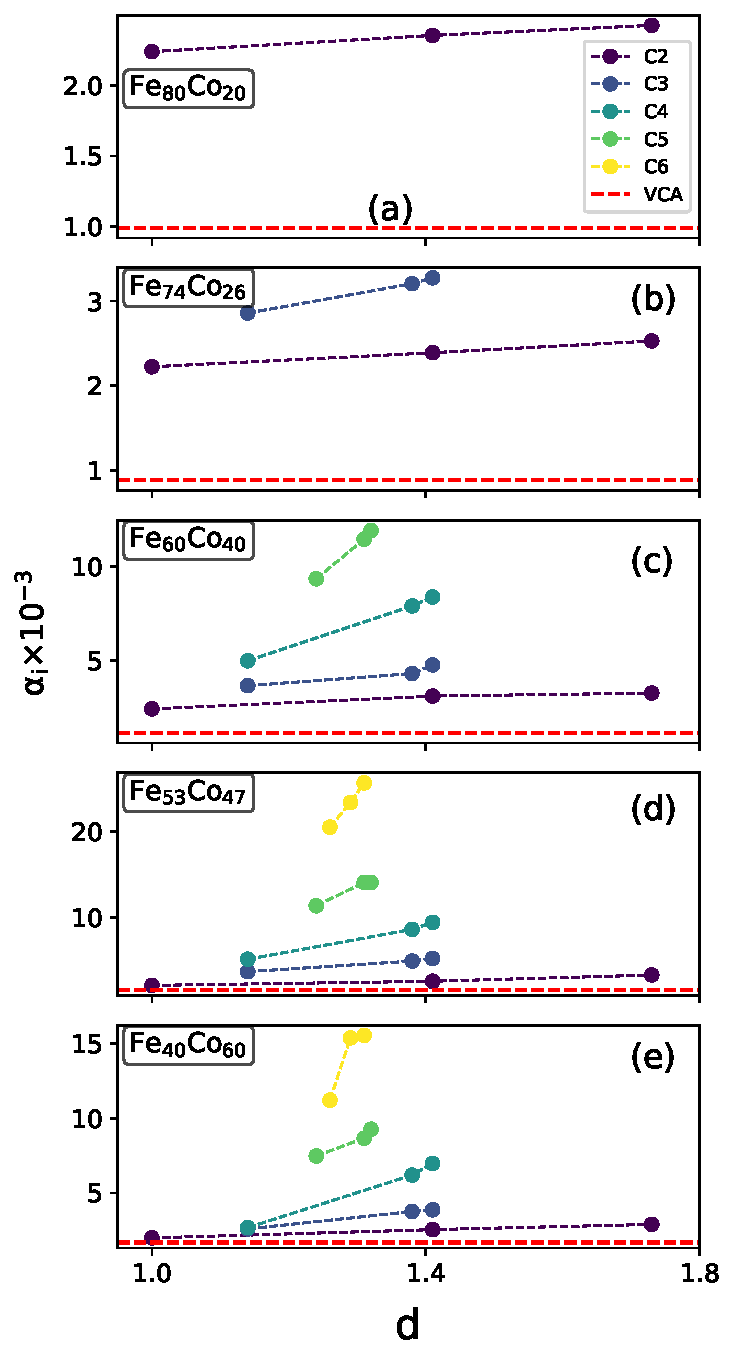
\includegraphics[width=0.9\columnwidth]{Fig6.pdf}
        \caption{
        Site-resolved damping parameter, $\alpha_i$ as a function of the normalized average Co interatomic distance $d$ as defined in Eq. \ref{eq:distance}, in units of $a_0$.     The filled circles in (a) to (e) show the effective damping of the clusters within C2-C6 groups for different FeCo alloy compositions. As a reference, the red dashed line shows the damping computed considering purely the VCA model.} 
        \label{fig3:alpha_distance} 
\end{figure}


\begin{table}[h]
\caption{Effective Gilbert damping variation $\Delta\alpha^{\text{eff}}$ as a function of \(n\) and composition \(x\) of Fe$_{100-x}$Co$_{x}$. $\Delta\alpha^{\text{max}}(\%)$, $\Delta n({E_f})^{\text{max}}(\%)$ represent the maximum variation of damping as well as density of states at the Fermi level between clusters within each Co composition, respectively.}
    \centering
    \begin{tabular}{cccccc}
        \toprule
        \toprule
    $n$ & & &$x$ $(\%)$ & & \\
         \toprule
           &   20 & 26 & 40 & 47 & 60 \\
        \midrule
        2 & 8 & 14 & 34 & 58 & 46 \\
        3 & -- & 15 & 30 & 41 & 50 \\
        4 & -- & -- & 68 & 83 & 161 \\
        5 & -- & -- & 27 & 24 & 24 \\
        6 & -- & -- & -- & 25 & 39 \\
        \midrule
        $\Delta\alpha^{\text{max}}$ & 8 & 47 & 387 & 1122 & 685 \\
        $\Delta n({E_f})^{\text{max}}$ & 3 & 22 & 115 & 195 & 150 \\
        \bottomrule
        \bottomrule
    \end{tabular}
    \label{tab:effdampvar}
\end{table}


Figure \ref{fig3:alpha_distance} shows $\alpha_i$ as a function of $d$, in different cluster groups C$n$ and alloy concentrations $x$. From those results, two observations can be made: first, $\Delta\alpha^{\textnormal{eff}}$ is in all cases positive and can reach values up to $161\%$ in C4 cluster group of Fe$_{40}$Co$_{60}$. Consequently, damping tends to increase with $d$ (see Table \ref{tab:effdampvar}).  

Second, the damping parameter depends on $n$, indicating a shift towards higher damping magnitudes as more Co atoms occupy 1st NN sites. Comparing the lowest and highest damping value among $n$ and $m$ for a fixed composition $x$, we observe a variation of up to $1122\%$ (or one order of magnitude) for $x=47$ between the configurations C2-1 and C6-3 (see Table \ref{tab:effdampvar}, bottom row, and Fig. \ref{fig:cluster} for an illustration of the referred clusters). This corroborates with the significance of the 1st NN Co atoms on the effective Gilbert damping in the central (or reference) site of the embedded cluster.


To delve deeper into damping's dependence on $d$, and to understand the relevant enhancement of damping in terms of the number of 1st NN Co atoms, we analyze the on-site $\alpha^{\textnormal{onsite}}$ (see Fig. \ref{fig:onsite_dos}, left column) and the nonlocal $\alpha^{\textnormal{nonlocal}}$ contributions. We obtain these two parameters from decomposing Eq. \ref{eq:damping_sum} into  $\alpha^{\textnormal{onsite}}=\alpha_{ii}$ and $\alpha^{\textnormal{nonlocal}}=\sum_{i\neq j}\alpha_{ij}$. In agreement with previous investigations \cite{PhysRevB.103.L220405, PhysRevMaterials.2.013801,PhysRevB.108.014433}, $\alpha^{\textnormal{onsite}}$ is positive and typically larger than $\alpha^{\textnormal{nonlocal}}$ for all clusters; for $3d$ materials such as FeCo, each $\alpha_{ij}$ is one order of magnitude lower than $\alpha_{ii}$, or more. Analogously to the effective damping, $\alpha^{\textnormal{onsite}}$ tends to increase with $d$ as well as $n$ and with similar variations. Surprisingly, $\alpha^{\textnormal{nonlocal}}$ changes sign and starts to be negative at $x>40\%$ for all $n$ and $m$. Different to the damping from pure VCA, where $\alpha^{\textnormal{nonlocal}}$ turns negative only at $x=60\%$, the nearest neighbor $\alpha_{ij}$'s drive the most significant contribution to the negative $\alpha^{\textnormal{nonlocal}}$ at $x>40\%$ (data not shown). Furthermore, $\alpha^{\textnormal{onsite}}$ seems to be more sensitive (by a factor of $\sim10$) in variations of $n$, $d$, and $x$ compared to $\alpha^{\textnormal{nonlocal}}$ and, thus, serves as the dominant component in the effective damping trends. The only exception to this general observation is the C2 cluster group, where onsite and nonlocal dampings are equally sensitive in variations of $d$ and for all Co concentrations $x$.
 

\begin{figure}[!ht]
\centering
        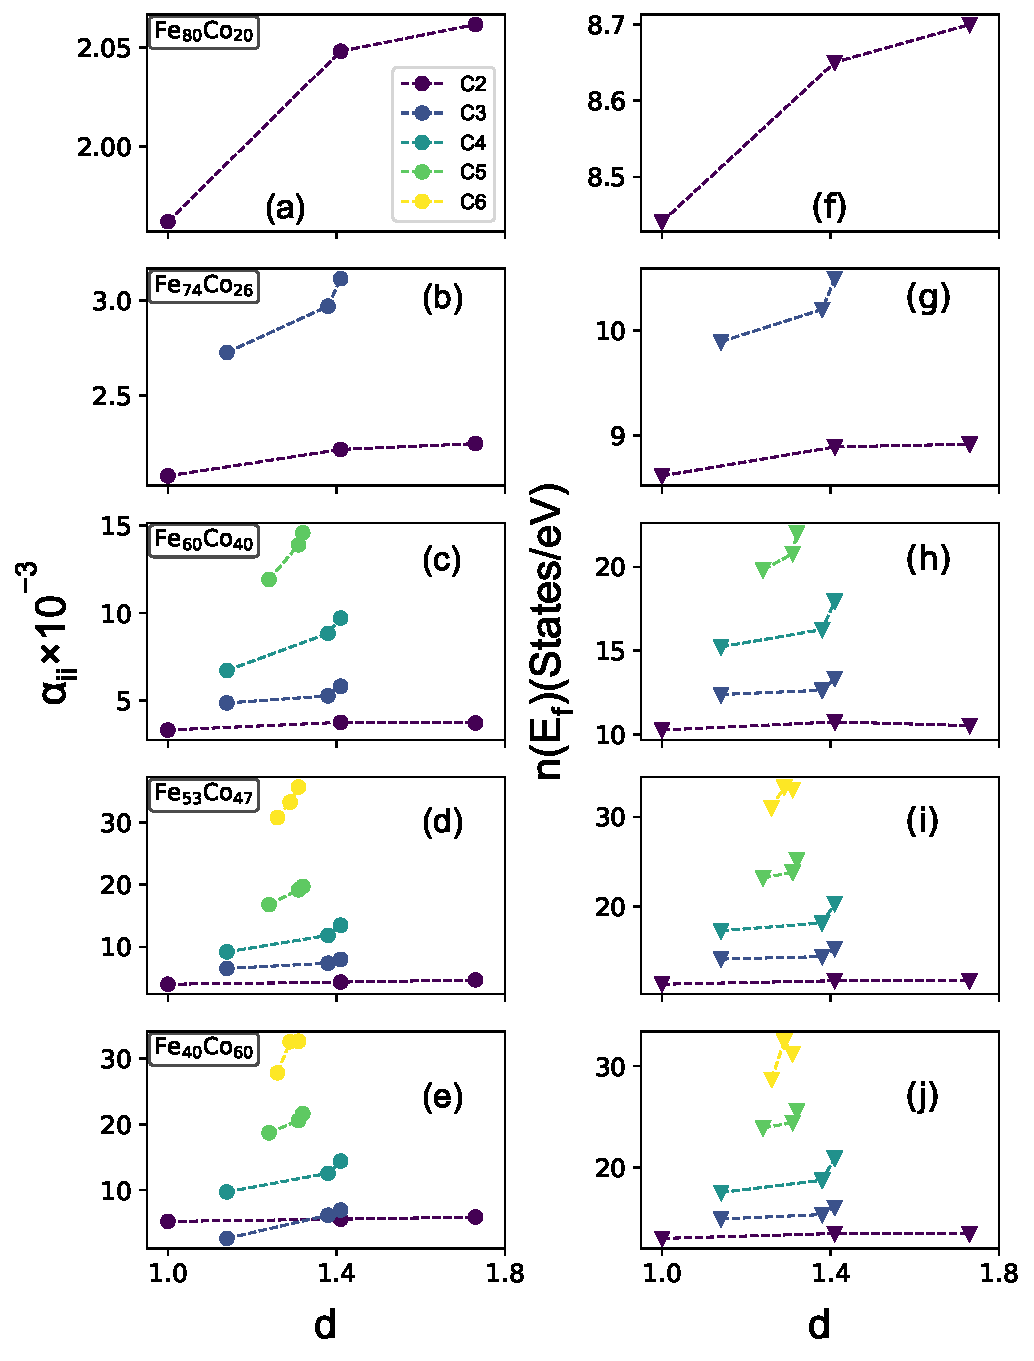
\includegraphics[width=1\columnwidth]{Fig7.pdf}
        \caption{Onsite damping $\alpha_{ii}$ (left panel) and density of states at the Fermi level $n(E_f)$ (right panel) as a function of the normalized average Co interatomic distance $d$ as defined in Eq. \ref{eq:distance}, in units of $a_0$, for different FeCo alloy compositions. The colors follow the scheme of Fig. \ref{fig3:alpha_distance}.}
        \label{fig:onsite_dos} 
\end{figure}



To further identify the electronic structure origin of the results in the effective, onsite, and nonlocal dampings, we link the first principles determined dampings to the approximate (or simplified) Kambersky’s formula for the relaxation of spin-dependent electronic populations  \cite{Kambersky1970},

\begin{equation}\label{eq:kambersky}
\begin{split}
\alpha = \frac{\gamma}{4 M_s} n({E_f})\xi^2(\delta g)^2\tau ,
\end{split}
\end{equation}
where $\gamma$ is the gyromagnetic ratio, $ M_s$ denotes the saturation magnetization, $n({E_f})$ represents the total density of states at the Fermi level, $\xi$ is the strength of spin-orbit coupling (SOC), $\delta g$ is the deviation of the $g$-factor from the free-electron value, 
and $\tau$ is the electron lifetime related to intrinsic scattering events with other degrees of freedom. 

The variation of the damping with respect to possible changes in $\xi$ is  negligible across all cluster groups, with the largest difference of less than $1\%$ found for the $3d$ states contribution to the SOC constant. 
Regarding $\tau$, its relation to the terminator and recursion levels of the Haydock method shows minor differences among clusters \cite{PhysRevB.103.L220405}, although the precise calculation of $\tau$ is beyond the scope of this study. In turn, the damping of different ferromagnetic materials have been associated with $(\delta g)^2$ before \cite{Oogane2006}, but the $\frac{m^{\textnormal{orb}}}{m^{\textnormal{spin}}}$ relation, within Kittel's first-order perturbation picture \cite{Shaw2021}, only changes subtly in each concentration $x$ (and specially within each C$n$ group). Explicitly, in all considered clusters, the central Co exhibits a spin moment of around $1.7\:\mu_B$ and an orbital moment of about $0.1\:\mu_B$, being in agreement with FeCo alloys and nanoclusters from previous works \cite{levzaic2007first,miranda2017dimensionality,gerasimov2021nature}. No clear trend is observed in spin and orbital moments with the average interatomic distance $d$. Nevertheless, an increase is noted with $n$, featuring the largest spin moment variation at $\sim1.8\%$ and the largest orbital moment variations at $\sim30-38\%$ for $x\geq40\%$, to be compared with $\Delta\alpha^{\textnormal{max}}$ --- i.e., giving somewhat a contribution but still not sufficient to explain the values shown in Table \ref{tab:effdampvar}. 

Therefore, in the scope of Eq. \ref{eq:kambersky}, the only quantity that remains to be analyzed is the total density of states (DOS) at the Fermi level. 
Significant correlation between $\alpha_i$ and $n({E_f})$ has been noted in this study and already in literature \cite{PhysRevB.94.214410}. It is shown in the second column of Fig.~\ref{fig:onsite_dos} that $n({E_f})$ exhibits a consistent enhancement trend with $d$ and $n$. The largest $\Delta n({E_f})$ found in each composition is shown in the bottom row of Table \ref{tab:effdampvar}, with qualitative agreement to the trends we observed for the effective damping. In detail, the local environment has a negligible impact on the spin-up channel's local DOS (LDOS), while it induces a shift in the spin-down channel towards lower energies, thus enhancing the corresponding LDOS at the Fermi level (data not shown).


Lastly, our findings reveal that the $\alpha_i$ is comparatively less sensitive on changes of $n$ for the Fe-centered clusters as well as on the local environment variation of the second nearest neighboring sites. Although the damping values of these clusters differ when compared to the pure VCA values, they are substantially lower than those observed in Co-centered cases and the cases varying in $d$ and $n$, respectively. For instance, when replacing the central Co atom with an Fe atom in Fe$_{53}$Co$_{47}$, and comparing the damping of clusters with different $n$, the maximum observed variation in damping – between the lowest and highest values – is $27\%$ (far less than in Co-centered cases). Additionally, our tests on several clusters with different second nearest neighbor environments show that the damping variations are negligible (less than $\sim5\%$). Furthermore, neither of these cases exhibit a clear trend in damping variation.
The underlying reason of this behavior is that the local environment impacts on $n({E_f})$ of Fe center clusters are negligible.

\subsection{Effective damping: towards the global frame}

\label{sec:global-perspective}

After analyzing the impact of specific Fe/Co configurations on Gilbert damping within a localized frame, we now discuss the EC-VCA results from a broader, more global perspective -- towards a random alloy model with short-range structure resolution. To this end, we proceed to calculate the average damping for each Co concentration.
Obviously, as detailed in Section \ref{subsec:local-effects-detailed}, as we move away from Co-poor alloys approaching Fe$_{50}$Co$_{50}$, the number of possible nonequivalent configurations greatly increases, which prevents a brute-force calculation of the precise average values for all $x$. As an illustration, we can briefly analyze the cases of $\rm Fe_{53}Co_{47}$ and $\rm Fe_{40}Co_{60}$. By utilizing a cluster expansion approach similar to that described in Refs. \cite{jiang2024influence, PhysRevB.81.245210, he2020atom}, 197 and 159 non-equivalent clusters are found for these compositions, respectively, without considering magnetic symmetry operations (SQA effect). Thus, a limited set has to be selected. We here choose to investigate one Fe-centered and one Co-centered cluster for each C$n$-$m$ group, including C0 and C1, for $0\%<x\leq40\%$; an example of this, applied to Co-centered clusters was already depicted in Fig. \ref{fig:cluster}. This approach yields a simplified and unbalanced average, which we argue is sufficiently representative to replicate the experimental trend.


Figure \ref{fig:damping_comparison} shows the average effective damping, obtained by using Eq. \ref{eq:total-damping}, considering both the Co-centered and Fe-centered clusters among the different concentrations. On one hand, quantitatively we observe that the average damping shown in Fig. \ref{fig:damping_comparison} is enhanced in comparison with the experimental results and even with VCA calculations. This, however, is expected from the unbalanced average model we choose and has two simple explanations: (\textit{i}) the averages are taken from incomplete sets of clusters; and (\textit{ii}) the high-$\alpha_i$ clusters are included. This can be clearly seen by incorporating the complete set value obtained in Section \ref{subsec:local-effects-detailed} for $\rm Fe_{87}Co_{13}$, denoted by a green star in Figure \ref{fig:damping_comparison}, and comparing it with the average value obtained by our established selection criteria. As Figure \ref{fig:damping_comparison} shows, the average represented by the green star is rather close to the experimentally observed value.

On the other hand, qualitatively we note that the experimental trend (with a minimum around $x\sim20\%$) and order of magnitude are well reproduced by the calculated values shown by black dots, despite the limited set and high-$\alpha_i$ clusters included. The error bars follow the percentage ($\sim11\%$) found in Section \ref{subsec:local-effects-detailed}, although we expect increased standard deviations as $x\rightarrow50\%$, specially because outliers with considerable $\Delta\alpha^{\textnormal{eff}}$ become more common in those alloy concentrations. Therefore, although unusually high $\alpha_i$ clusters can emerge as a result of chemical disorder, those cases are hidden in real intrinsic damping measurements by statistical averages. This makes the local scenario described in Section \ref{subsec:damping variation} consistent with FMR experiments again.  



\begin{figure}[!ht]
\centering
        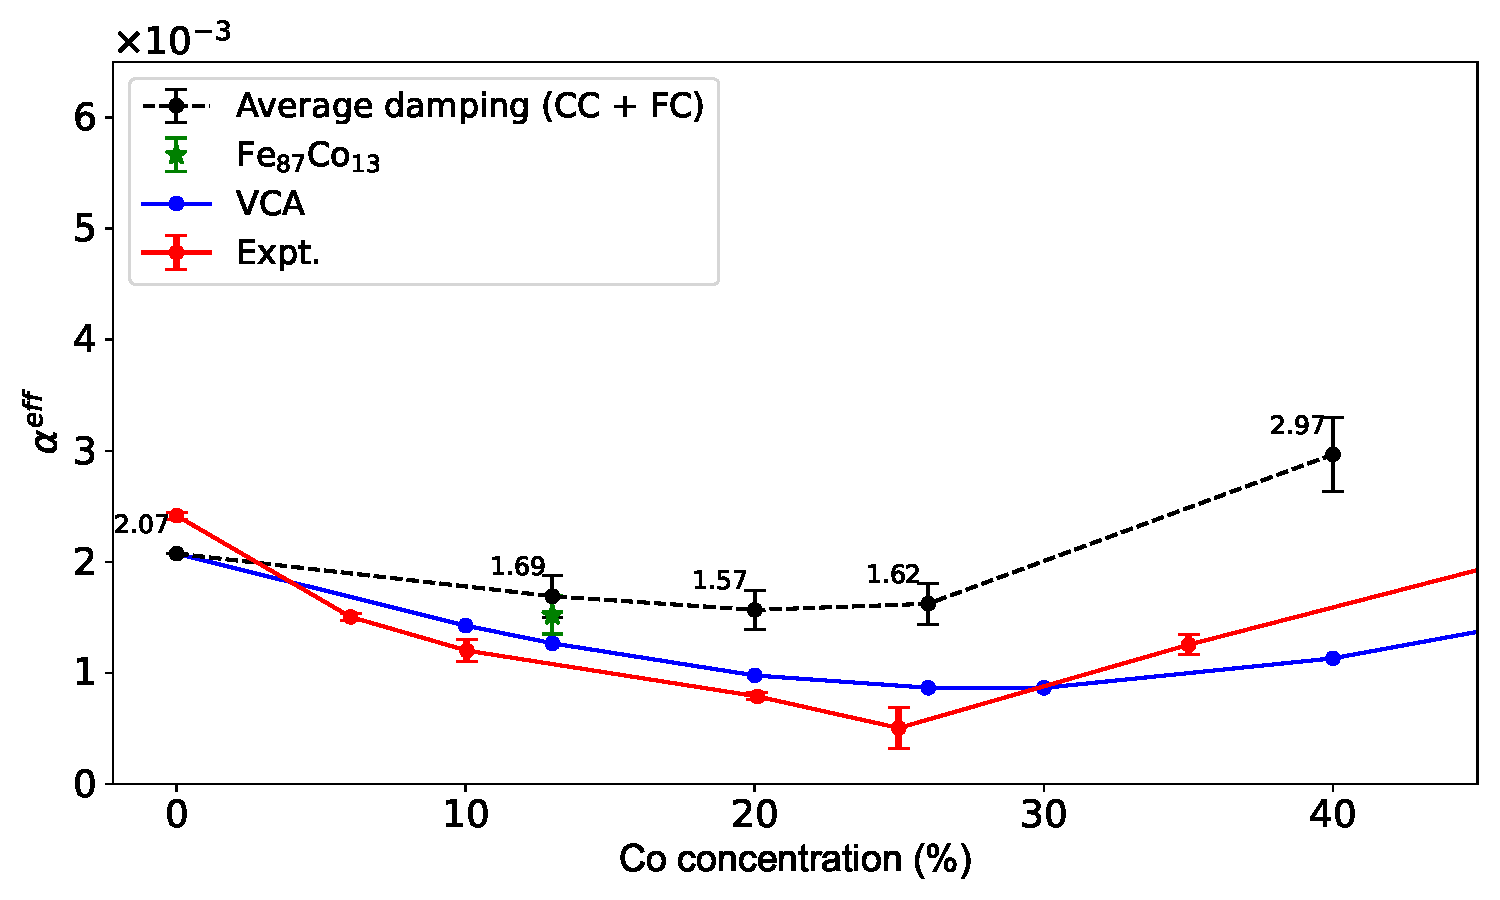
\includegraphics[width=1\columnwidth]{Fig8.pdf}
        \caption{The effective intrinsic damping as a function of Co concentration. The averages (black dots) are performed over all considered Fe-centered and Co-centered clusters within each C$n$-$m$ group, and calculated in the FMR regime by Eq. \ref{eq:effective-alpha-parameter}. The blue and red dots show, respectively, the damping obtained from pure VCA calculations and experimental results from Ref. \cite{Schoen2016}. The average value for $\rm Fe_{87}Co_{13}$ obtained in Section \ref{subsec:local-effects-detailed} is depicted by the green star. Error bars are calculated as $\sim11\%$ of each value, as a result of the standard deviation obtained in the $\rm Fe_{87}Co_{13}$ case (see text). Lines are guides for the eyes.} 
        \label{fig:damping_comparison} 
\end{figure}